
\documentclass[11pt]{article}

\usepackage{common}
\title{HW4: Word Segmentation}
\author{Jeffrey Ling \\ jling@college.harvard.edu \and Rohil Prasad \\ prasad01@college.harvard.edu }
\begin{document}

\maketitle{}
\section{Introduction}

In this assignment, we examine the problem of word segmentation. Given a string of characters without spaces, we want to determine where we can insert spaces to segment the string into words. 

We implement and discuss several approaches to word segmentation in this paper, all trained on a portion of the Penn Treebank. Our first class of models are hidden Markov models with emission distributions given by an n-gram count model and an adaptation of Bengio's neural network language model (NNLM). Our second class of models are recurrent neural networks (RNNs), namely the Long Short Term Memory (LSTM) network and the Gated Recurrent Unit (GRU) network. Furthermore, we attempt to optimize the evaluation algorithms used to construct segmentations given a model. For the Markovian models, we use a dynamic programming algorithm which greatly improves predictive accuracy. We also make a small adjustment to the RNN evaluation algorithm that the performance of these models as well. 

In Section 2, we give a formal description of our problem and establish our notation. In Section 3, we give detailed descriptions of the algorithms listed above. In Section 4, we present our experimental results. In Section 5, we discuss our findings.

\section{Problem Description}

Assume our training corpus consists of a sequence of characters $c_1, c_2, \dots, c_N$ where $c_i$ is drawn from a vocabulary $\mathcal{V}$ for every $i$. We use $<sp> \in \mathcal{V}$ to denote the space character. 

Our training data represents this corpus as a set of pairs $(c_i, y_i)$ for $i \in \{1, \dots, N\}$. The output variable $y_i$ is set to be equal to $1$ if the next character $c_{i+1}$ is not a space, and $2$ if it is a space. By default, we set $y_N = 1$ since $c_N$ is clearly not followed by a space. 

Calculating a word segmentation is equivalent to taking an input sequence of characters $\mathbf{c}' = c_1c_2\dots c_M$ of characters as input and outputting a sequence $y_1y_2\dots y_M$, where $y_i = 2$ if we insert a space after $c_i$ and $1$ if not. 

We determine the \emph{best} word segmentation by finding the sequence $y_1y_2\dots y_M$ that maximizes the joint probability function $f(c_1, \dots, c_M, y_1, \dots, y_M) = p(c_1, \dots, c_M, y_1, \dots, y_M)$. 

For the approaches we are considering, this requires us to train a model that will take an input character $c$ and output the probability that the next character is a space. Then, we apply an evaluation algorithm at test time to generate the best sequence. 

\subsection{Evaluation}

We evaluate our models on two validation sets. These validation sets contain the same characters, but one already contains spaces while the other does not. 

First, note that our model is essentially a language model, taking in a character and outputting a simple distribution on the next character. Therefore, we can calculate perplexity over the validation set with spaces. This is equal to the exponential of the average negative log likelihood. Since we only have two classes, the perplexity is at most $2$. 

For our second validation set, we can run our model and evaluation algorithm to get a word segmentation over the entire set. Here, we keep track of the number of spaces inserted into each sentence and compute the mean squared error of these numbers with respect to the provided answers for each sentence. 

\section{Model and Algorithms}

\subsection{Markovian Models}

The key to these models is the Markov assumption, which states that $p(y_i | y_1, \dots, y_{i-1}) = p(y_i | y_{i-k+1}, \dots, y_{i-1})$ for some fixed $k$. This allows us to get a simple expression for the joint probability that we can calculate using either a count-based model or a neural network model. 

We can expand out the joint probability as 
\begin{align*}
  p(c_1, \dots, c_M, y_1, \dots, y_M) &= p(c_1, \dots, c_M | y_1, \dots, y_M)p(y_1, \dots, y_M) \\
  &= \prod_{i=1}^M p(c_i | c_1, \dots, c_{i-1}, y_1, \dots, y_M)p(y_i | y_1, \dots, y_{i-1}) \\ 
  &= \prod_{i=1}^M p(c_i | c_1, \dots, c_{i-1}, y_1, \dots, y_M)p(y_i | y_{i-k+1}, \dots, y_{i-1}) \\
\end{align*}

\subsubsection{Count Model}

\subsubsection{Neural Network Linear Model}

We use Bengio's neural network model like last assignment. It aim to directly learn a function from the context $c_{i-k+1}c_{i-k+2}\dots c_i$ to $y_i$. We have parameters
\begin{itemize}
  \item $W_0 \in \mathbb{R}^{|\mathcal{V}| \times d_{in}|}$, a lookup table of character embeddings
  \item $W_1 \in \mathbb{R}^{kd_{in} \times d_{hid}}$, $b_1 \in \mathbb{R}^{d_{hid}}$,
  \item $W_2 \in \mathbb{R}^{d_{hid} \times |\mcV|}$, $b_2 \in \mathbb{R}^{2}$
\end{itemize}

First, the character context is transformed into character embeddings by multiplying with $W_0$, and then concatenated to get a vector $\mathbf{x}_0$ of size $k \cdot d_{in}$. Then, we get a size $2$ vector of scores
$$\mathbf{z} = \text{tanh}(\mathbf{x}_0W_1 + b_1)W_2 + b_2 \in \mathbb{R}^2$$

Finally, we can force a probability distribution by taking the softmax $\hat{y} = \text{softmax}(\mathbf{z})$. Then, we have the probability that the next word is a space is $P(y_i = 2) = \hat{y}_2$, while the probability that it is not a space is $P(y_i = 1) = \hat{y}_1$. 

\subsection{Recurrent Neural Networks}

Our recurrent neural networks have the following parameters:
\begin{itemize}
  \item $W_0 \in \mathbb{R}^{|\mathcal{V}| \times d_{in}}$,
  \item $\mathbf{s}_0 \in \mathbb{R}^{d_{hid}}$, the initial hidden state,
  \item $R: \mathbb{R}^{d_{hid}} \times \mathbb{R}^{d_{in}} \to \mathbb{R}^{d_{hid}}$, a parameterized state transition function,
  \item $W_1: \mathcal{R}^{d_{hid}} \to \mathbb{R}^2$, $b_1 \in \mathbb{R}^{2}$
\end{itemize}

The exact definition of $R$ depends on the type of RNN we are using. All of our RNNS are\textbf{transducer} RNNs, meaning that they consume an input sequence $c_1, \dots, c_M$ of characters and output a sequence $\hat{y}_1, \dots, \hat{y}_M$, where $\hat{y}_i = p(y_i | c_i, c_{i-1}, \dots, c_1)$. 

\subsubsection{Long Short Term Memory Network}

We use the LSTM model of Hochreiter and Schmidhuber, illustrated below:

\begin{center}
  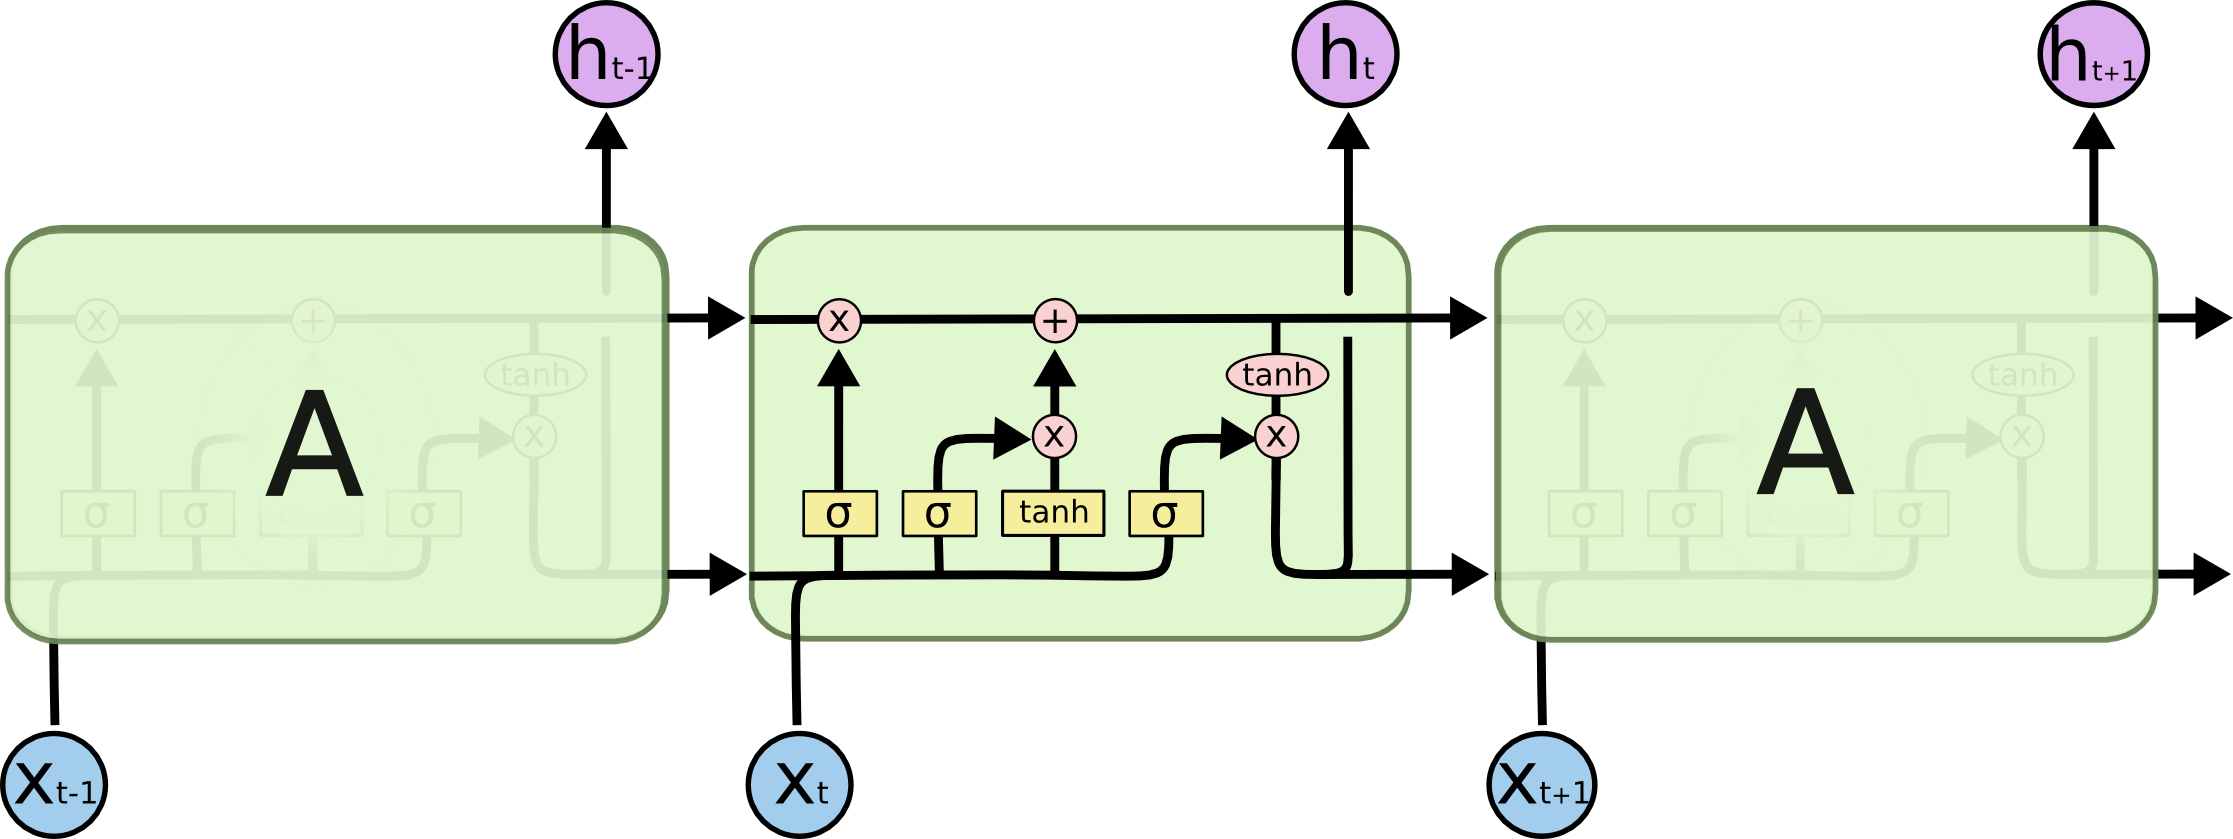
\includegraphics[width=0.5\textwidth]{LSTM3-chain.png}
\end{center}

Formally, this requires the introduction of some new parameters
\begin{itemize}
  \item $W^{xi} \in \mathbb{R}^{d_{in} \times d_{hid}}$, $W^{si} \in \mathbb{R}^{d_{hid} \times d_{hid}}$, $b^i \in \mathbb{R}^{d_{hid}}$, 
  \item $W^{xi} \in \mathbb{R}^{d_{in} \times d_{hid}}$, $W^{sj} \in \mathbb{R}^{d_{hid} \times d_{hid}}$, $b^j \in \mathbb{R}^{d_{hid}}$,
  \item $W^{xi} \in \mathbb{R}^{d_{in} \times d_{hid}}$, $W^{sf} \in \mathbb{R}^{d_{hid} \times d_{hid}}$, $b^f \in \mathbb{R}^{d_{hid}}$,
  \item $W^{xi} \in \mathbb{R}^{d_{in} \times d_{hid}}$, $W^{so} \in \mathbb{R}^{d_{hid} \times d_{hid}}$, $b^o \in \mathbb{R}^{d_{hid}}$,
  \item $\mathbf{C}_0 \in \mathbb{R}^{d_{hid}}$, the initial cell state
\end{itemize}

Let $c_i$ be our input character, and let $\mathbf{C}_{i-1}$ and $\mathbf{s}_{i-1}$ be the previously calculated cell and hidden states, respectively. First, we transform $c_i$ into a vector $\mathbf{x}_i$ of size $d_{in}$ by multiplying it by $W_0$. Then, we calculate the four following vectors
\begin{align*}
  \mathbf{i} &= \text{tanh}(\mathbf{x}_iW^{xi} + \mathbf{s}_{i-1}W^{si} + b^i \\
  \mathbf{j} &= \sigma(\mathbf{x}_iW^{xj} + \mathbf{s}_{i-1}W^{sj} + b^j \\
  \mathbf{i} &= \sigma(\mathbf{x}_iW^{xf} + \mathbf{s}_{i-1}W^{sf} + b^f \\
  \mathbf{i} &= \text{tanh}(\mathbf{x}_iW^{xo} + \mathbf{s}_{i-1}W^{so} + b^o \\
\end{align*}
and combine them to produce the new cell state and hidden state
\begin{align*}
  \mathbf{C}_i &= \mathbf{j} \odot \mathbf{i} + \mathbf{f} \odot \mathbf{C}_{i-1} \\
  \mathbf{s}_i &= R(\mathbf{s}_{i-1}, \mathbf{x}_i) = \text{tanh}(\mathbf{C}_i) \odot \mathbf{o}
\end{align*}
Then, we multiply $\mathbf{s}_i$ by $W_1$ to produce an output vector $\mathbf{z}_i$ of size $2$. Finally, we force a probability distribution by taking the softmax to get the desired output $\hat{y}_i = \text{softmax}(\mathbf{z}_i)$. 

\subsubsection{Gated Recurrent Unit Network}

We use the GRU model of Cho et al. This model requires the following parameters in addition to the generic RNN parameters
\begin{itemize}
  \item $W^{xt} \in \mathbb{R}^{d_{in} \times d_{hid}}$, $W^{st} \in \mathbb{R}^{d_{hid} \times d_{hid}}$, $b^t \in \mathbb{R}^{d_{hid}}$, 
  \item $W^{xr} \in \mathbb{R}^{d_{in} \times d_{hid}}$, $W^{sr} \in \mathbb{R}^{d_{hid} \times d_{hid}}$, $b^r \in \mathbb{R}^{d_{hid}}$, 
  \item $W^x \in \mathbb{R}^{d_{in} \times d_{hid}}$, $W^s \in \mathbb{R}^{d_{hid} \times d_{hid}}$, $b \in \mathbb{R}^{d_{hid}}$
\end{itemize}

Let $c_i$ be our input character, and let $\mathbf{s}_{i-1}$ be the previously calculated hidden state. First, we transform $c_i$ into a vector $\mathbf{x}_i$ of size $d_{in}$ by multiplying it by $W_0$. Then, we calculate the following three vectors
\begin{align*}
  \widetilde{\mathbf{h}} &= \text{tanh}(\mathbf{x}_iW^{x} + (\mathbf{r} \odot \mathbf{s}_{i-1})W^s + b) \\
  \mathbf{r} &= \sigma(\mathbf{x}_iW^{xr} + \mathbf{s}_{i-1}W^{sr} + b^r) \\
  \mathbf{t} &= \sigma(\mathbf{x}_iW^{xt} + \mathbf{s}_{i-1}W^{st} + b^t)
\end{align*}
and combine them to produce the new hidden state
\begin{align*}
  \mathbf{s}_i &= R(\mathbf{s}_{i-1}, \mathbf{x}_i) = (1 - \mathbf{t}) \odot \widetilde{\mathbf{h}} + \mathbf{t} \odot \mathbf{s}_{i-1}
\end{align*}
Then, we multiply $\mathbf{s}_i$ by $W_1$ to produce an output vector $\mathbf{z}_i$ of size $2$. Finally, we force a probability distribution by taking the softmax to get the desired output $\hat{y}_i = \text{softmax}(\mathbf{z}_i)$. 
\subsection{Evaluation Algorithms}

We have three different algorithms that we use to take a model and use it to predict a sequence $y_1\dots y_M$ for an input sequence $c'_1\dots c'_M$. The first two are a greedy algorithm and a dynamic programming algorithm for our Markovian models. The last one is a greedy algorithm for our RNN models. In all of them, we will denote our model by a function $f$ from the input space to the space/non-space probability distribution. 

\subsubsection{Markovian Greedy}

The algorithm is given formally. It simply consists of greedily predicting each $y_i$ and recording how many $y_i = 2$ per sentence. 

\begin{algorithmic}
  \Procedure{MarkovGreedy}{$c'_1, \dots, c'_M$, $f$}
    \State{$sn \leftarrow 1$}
    \Comment{Set sentence number to $1$}
    \State{$S = \{\}$}
    \Comment{Initialize empty dictionary}
    \For{$i \in 1, \dots, M$}
      \If{$c'_i = </s>$}
        \State{$sn \leftarrow sn + 1$}
        \State{$S[sn] \leftarrow 0$}
        \Comment{Increment sentence number at end of sentence}
      \EndIf{}
      \State{$y \leftarrow f(c'_i)_2$}
      \Comment{Feed $c'_i$ into the model}
      \If{$y \geq 1/2$}
        $S[sn] \leftarrow S[sn] + 1$
      \EndIf{}
    \EndFor{}
    \Return{$S$}
  \EndProcedure{}
\end{algorithmic}

\subsubsection{Markovian Dynamic Programming}

\subsubsection{RNN Greedy}

The algorithm is given formally below. In plain language, we simply feed in each character one at a time to our RNN. If the RNN predicts a space, we record that in our output dictionary and feed the space in and then continue to the next character. 

\begin{algorithmic}
  \Procedure{RNNGreedy}{$c'_1, \dots, c'_M$, $f$, $\mu$, $<sp>$, $</s>$}
    \State{$i \leftarrow 1$}
    \State{$sn \leftarrow 1$}
    \Comment{Set sentence number to $1$}
    \State{$S = \{\}$}
    \Comment{Initialize empty dictionary}
    \State{$S[sn] = 0$}
    \While{$i \leq M$}
      \If{$c'_i = </s>$}
        \State{$sn \leftarrow sn + 1$}
        \State{$S[sn] \leftarrow 0$}
        \Comment{Increment sentence number at end of sentence}
      \EndIf{}
      \State{$y \leftarrow f(c'_i)_2$}
      \Comment{Feed $c'_i$ into the model}
      \If{$y \geq \mu$}
        \State{$y \leftarrow f(<sp>)$}
        \State{$S[sn] = S[sn] + 1$}
        \Comment{Feed a space into the model}
      \EndIf{}
      \State{$i \leftarrow i+1$}
    \EndWhile{}
  \Return{$S$}
  \EndProcedure{}
\end{algorithmic}

\section{Experiments}

The table below documents the training set perplexity, validation set perplexity, and training time for each of our models. The training time for the NNLM and RNN models are given per epoch. 

\begin{center}
  \begin{tabular}{| c | c | c | c |}
    \hline Model & Train Perplexity & Valid Perplexity & Training Time \\
    \hline Count & & & \\
    NNLM & & & \\
    LSTM & & & \\
    GRU & & & \\
    \hline
  \end{tabular}
\end{center}

For the NNLM and RNN models, we also plot the train/valid perplexities per epoch to verify that our models are training properly. 

We also recorded the MSE of the spaces per sentence predictions of our models with each evaluation algorithm. 

\begin{center}
  \begin{tabular}{| c | c | c |}
    \hline Model & Algorithm & MSE \\
    \hline Count & Greedy & \\
    & DP & \\
    NNLM & Greedy & \\
    & DP & \\
    LSTM & Greedy & \\
    GRU & Greedy & \\
    \hline
  \end{tabular}
\end{center}

The MSE for RNN greedy is that for $\mu = 0.3$, which was optimized by grid search on an LSTM trained for $20$ epochs. The results are given in the table below. 

\begin{center}
\begin{tabular}{| c | c |}
  \hline $\mu$ & MSE \\
  \hline $0.1$ & 19.1\\
  $0.2$ & 7.7\\
  $0.3$ & 5.4\\
  $0.4$ & 6.3\\
  $0.5$ & 10.9\\
  $0.6$ & 18.6\\
  $0.7$ & 33.6\\
  $0.8$ & 59.8\\
  $0.9$ & 144.4\\
  \hline
\end{tabular}
\end{center}

\section{Conclusion}



\bibliographystyle{apalike}
\bibliography{writeup}

\end{document}
